\documentclass[11pt]{article}

\usepackage[margin=1in]{geometry}
\usepackage[T1]{fontenc}
\usepackage[utf8]{inputenc}
\usepackage{lmodern}
\usepackage{microtype}
\usepackage{amsmath,amssymb}
\usepackage{booktabs}
\usepackage{graphicx}
\usepackage{xcolor}
\usepackage{hyperref}
\usepackage{enumitem}

\hypersetup{
  colorlinks=true,
  linkcolor=blue!50!black,
  urlcolor=blue!50!black,
  citecolor=blue!50!black
}

\title{Symmetry-Aware Operator Learning for the Bounded Burgers Benchmark}
\author{Autoresearch Notes}
\date{March 24, 2026}

\begin{document}
\maketitle

\section{Problem Setup}
We study operator learning for the one-dimensional viscous Burgers equation on the fixed bounded domain
\[
u_t + u\,u_x - \nu u_{xx} = 0,
\qquad x \in [-1,1], \quad t \in [0,1],
\]
with homogeneous Dirichlet boundary conditions
\[
u(-1,t)=u(1,t)=0.
\]
The surrogate takes as input the viscosity $\nu$ and an initial condition $u_0(x)$ sampled from the fixed hierarchical Gaussian random field prior used by the benchmark harness, and predicts the full spatio-temporal field $u(x,t)$.

The symmetry search started from the already-strong large-run architecture and asked a narrower question: can we improve the surrogate by encoding the \emph{actual} symmetries of the bounded problem directly into the neural representation?

\section{Which Symmetries Survive the Bounded Benchmark?}
The important distinction is between symmetries of the infinite-domain PDE and symmetries that still survive after imposing a finite interval, fixed coordinates, zero Dirichlet boundaries, and a fixed data prior.

\subsection{Exact symmetry used by the search}
The main exact symmetry of this bounded benchmark is the combined mirror-sign transform
\[
\mathcal{S}[u](x,t) = -u(-x,t).
\]
If $u(x,t)$ solves Burgers with viscosity $\nu$, then the transformed field $\tilde u(x,t)=-u(-x,t)$ also solves the same equation with the same viscosity, provided the initial condition is transformed as
\[
\tilde u_0(x) = -u_0(-x).
\]
This symmetry is compatible with the boundary conditions because
\[
\tilde u(\pm 1,t) = -u(\mp 1,t)=0.
\]

This is the symmetry the symmetry run ultimately exploited:
\begin{itemize}[leftmargin=1.5em]
\item parity-aware trunk features so the coordinate encoder distinguishes even and odd responses under $x \mapsto -x$,
\item branch inputs that expose both $u_0(x)$ and its mirror-sign partner,
\item exact reflection-sign projection at prediction time,
\item an explicit envelope that preserves the bounded Dirichlet walls.
\end{itemize}

\subsection{Symmetries that do \emph{not} survive here}
Several plausible transformations do not survive this benchmark:
\begin{itemize}[leftmargin=1.5em]
\item \textbf{Reflection only:} $u(x,t)\mapsto u(-x,t)$ is not a symmetry because the nonlinear advection term changes sign incorrectly.
\item \textbf{Global sign only:} $u(x,t)\mapsto -u(x,t)$ is also not a symmetry for the same reason.
\item \textbf{Translation:} broken by the fixed interval $[-1,1]$ and the zero Dirichlet walls.
\item \textbf{Scaling:} broken by the fixed domain, fixed time interval, and viscosity parameterization of the benchmark.
\item \textbf{Rotation:} not relevant for this one-dimensional space-time setting.
\end{itemize}

The search validated these distinctions empirically: the reflection-only and sign-only projections produced catastrophic errors, while the mirror-sign construction improved the model immediately.

\section{What Changed in the Network?}
The key result is that the best symmetry-aware model did \emph{not} win by making the network much larger. It kept the same DeepONet skeleton and changed the representation so the correct bounded-domain symmetry is built in.

\begin{table}[ht]
\centering
\begin{tabular}{@{}lll@{}}
\toprule
Component & Symmetry Baseline & Best Symmetry Model \\
\midrule
Model family & DeepONet & DeepONet \\
Branch / trunk & \texttt{resmlp} / \texttt{mlp} & \texttt{resmlp} / \texttt{mlp} \\
Hidden width & $640 / 640$ & $640 / 640$ \\
Latent size & $448$ & $448$ \\
Coordinate encoding & \texttt{fourier} & \texttt{fourier\_parity} \\
Branch input mode & raw & \texttt{reflection\_sign\_split} \\
Symmetry mode & none & \texttt{reflection\_sign\_projection} \\
Boundary mode & none & \texttt{quadratic\_dirichlet} \\
Fourier features / scale & $96 / 3.0$ & $96 / 3.0$ \\
Parameter count & $5.296$M & $5.502$M \\
\bottomrule
\end{tabular}
\caption{Baseline versus best kept symmetry-aware architecture.}
\end{table}

Structurally, the winning changes were:
\begin{enumerate}[leftmargin=1.5em]
\item Replace generic Fourier trunk features with parity-aware trunk features.
\item Replace raw branch input with a branch representation that explicitly exposes the mirror-sign partner.
\item Enforce exact reflection-sign equivariance at prediction time.
\item Multiply the predicted field by an even quadratic envelope so the network respects the bounded Dirichlet walls by construction.
\end{enumerate}

The parameter count only increased by about $3.9\%$ ($5.296$M $\rightarrow$ $5.502$M). The improvement came from encoding the right structure, not from scaling capacity again.

\section{Empirical Outcome}
For the symmetry run alone, the control baseline achieved
\[
\mathrm{val\_rel\_l2} = 1.667797\times 10^{-2},
\]
while the best kept symmetry-aware model achieved
\[
\mathrm{val\_rel\_l2} = 9.743770\times 10^{-3}.
\]
That is a $1.71\times$ improvement, or a $41.6\%$ reduction in validation error.

The best kept configuration was commit \texttt{d4f60d6}, described in the run ledger as:
\begin{quote}
exact reflection-sign equivariance plus an even Dirichlet envelope that preserves mirror-sign symmetry on the finite interval.
\end{quote}

Several follow-up ideas were useful negative results:
\begin{itemize}[leftmargin=1.5em]
\item raw coordinates were worse than parity-aware features,
\item deterministic Dirichlet parity harmonics were worse than random parity-aware Fourier features,
\item factorized trunk irreps and latent-space equivariant projection did not beat the simpler output-space projection,
\item quartic and cosine wall envelopes both trailed the simpler quadratic envelope,
\item a wider Fourier basis and a larger mirrored latent basis came close but still lost.
\end{itemize}

\begin{figure}[ht]
\centering
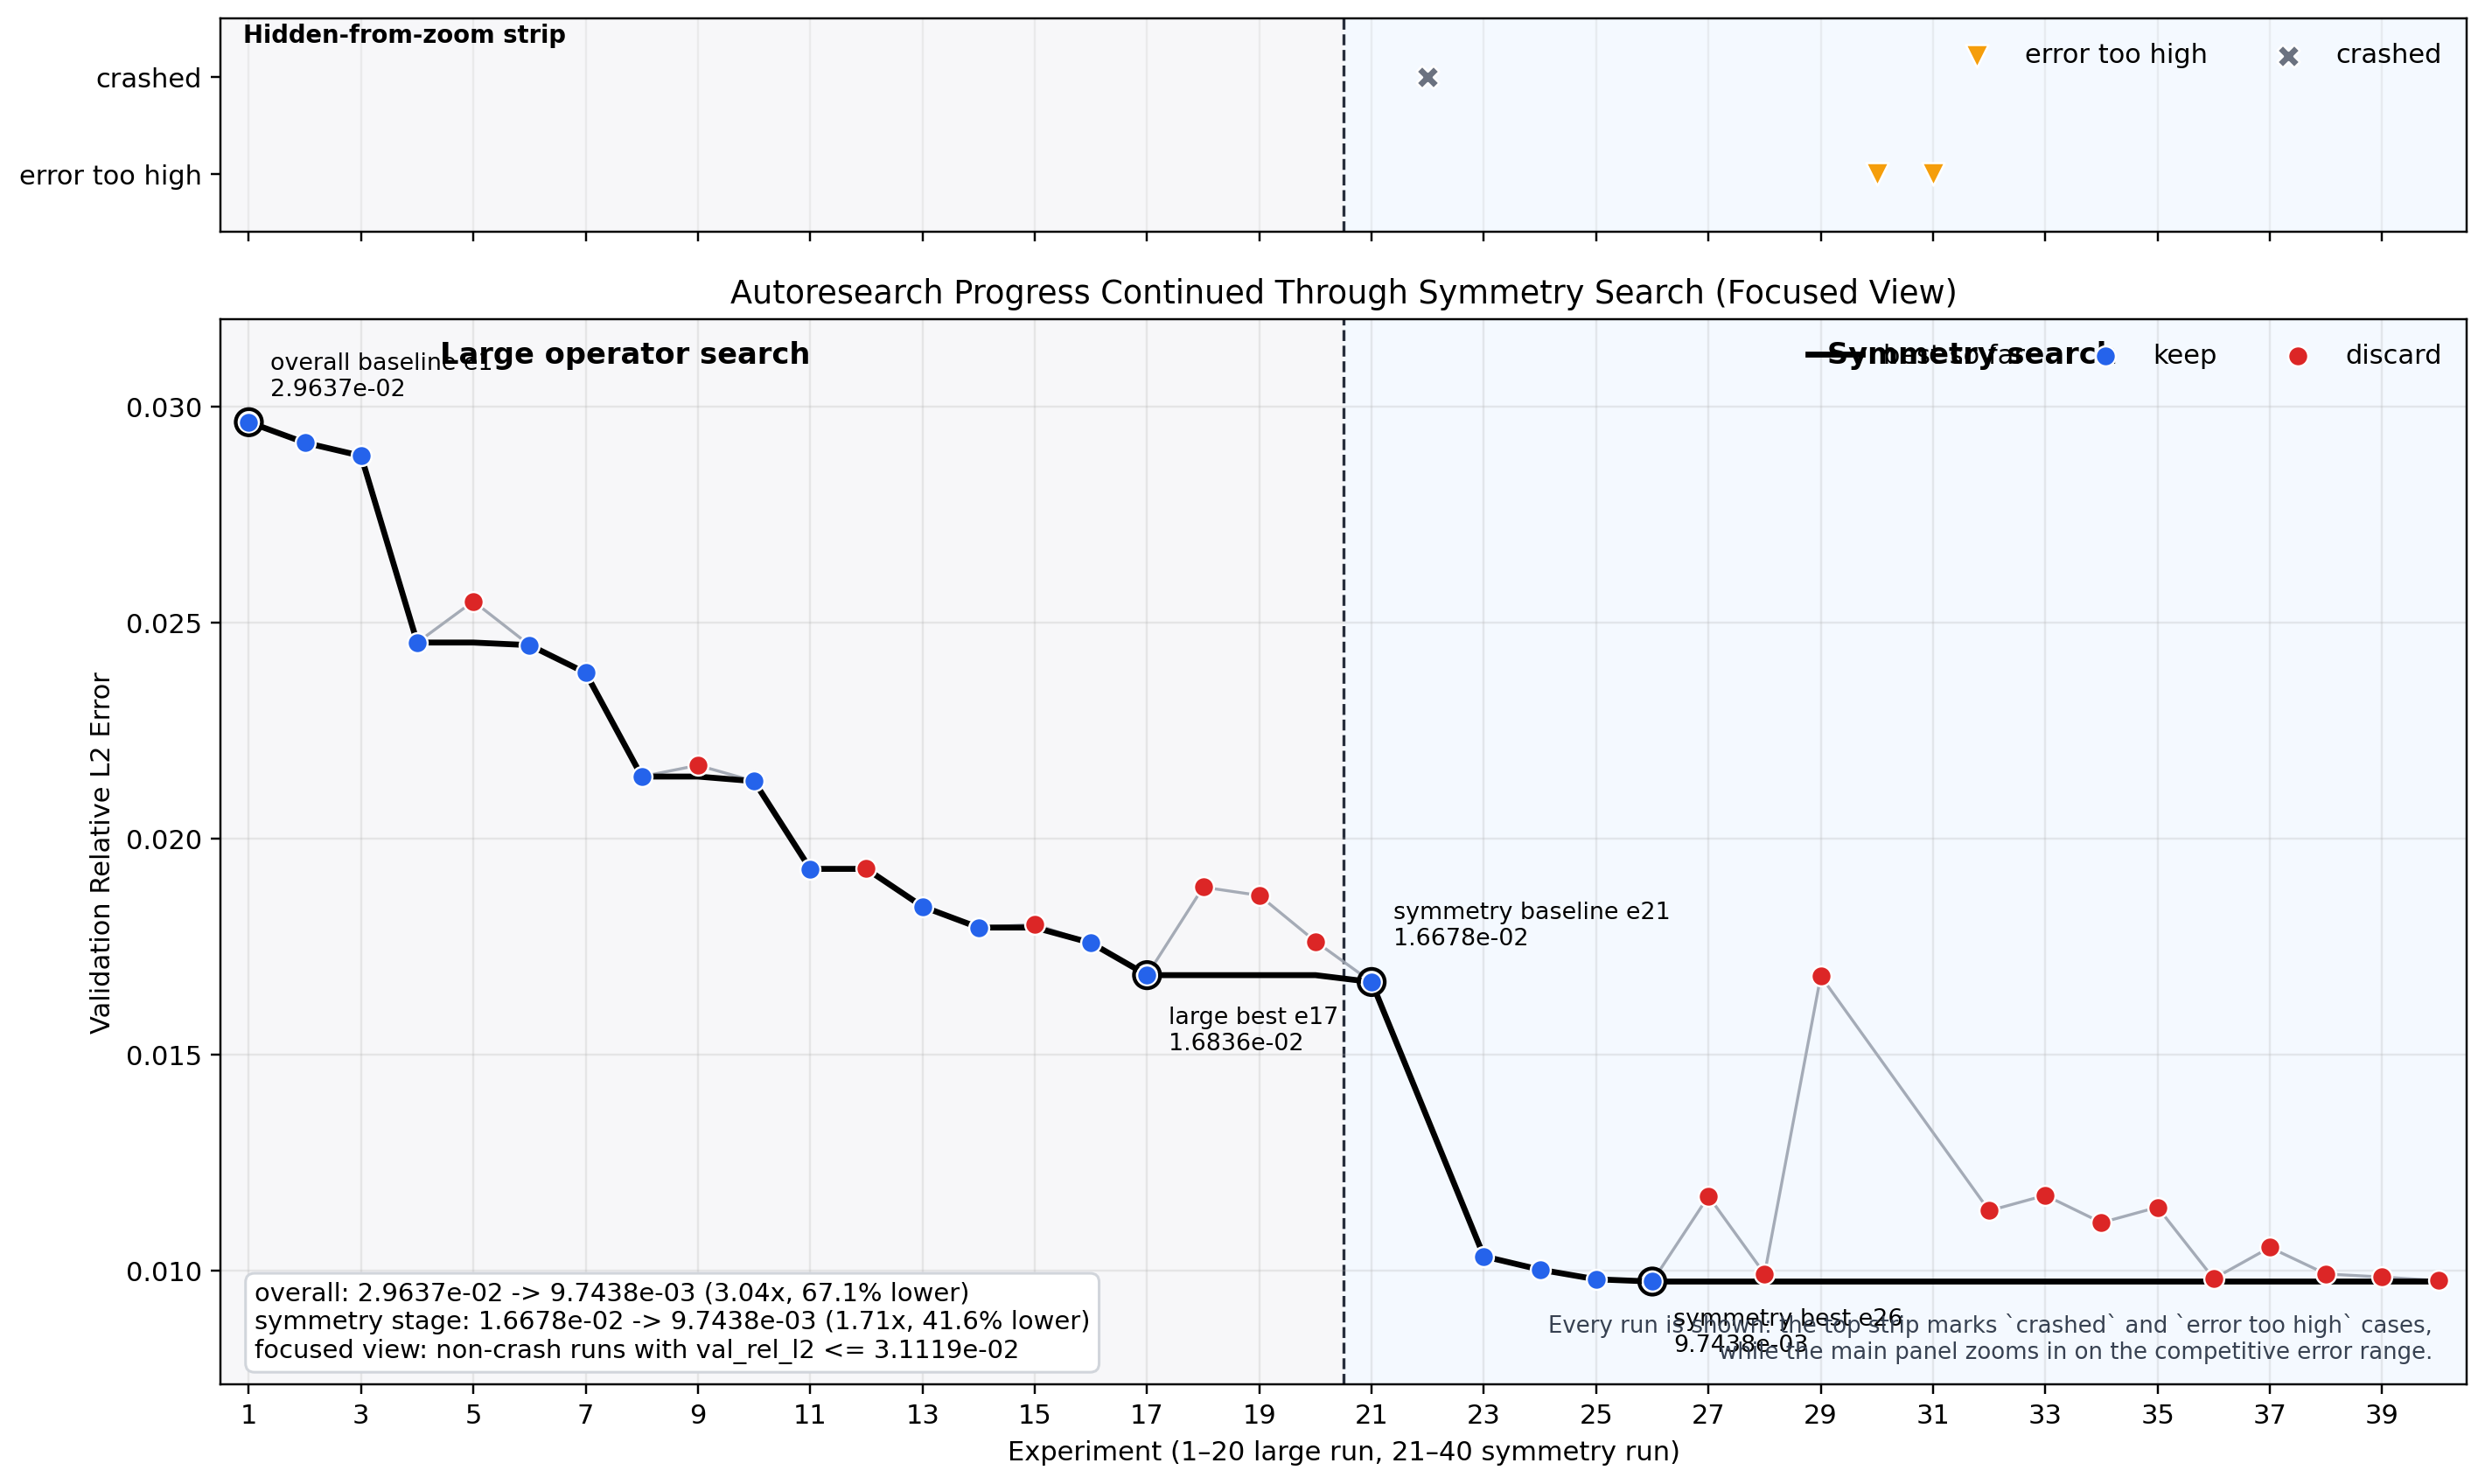
\includegraphics[width=\textwidth]{figure_progress_continued.png}
\caption{Continued progress curve across the earlier large-run search and the later symmetry-focused search. The top strip marks noncompetitive runs explicitly as \texttt{crashed} or \texttt{error too high}; the main panel zooms into the competitive region.}
\end{figure}

\section{Takeaway}
The symmetry search suggests a clear lesson: for this bounded Burgers operator problem, the right inductive bias is not ``more network'' so much as ``more correct structure.'' The winning model kept the same overall DeepONet shape and almost the same scale, but changed how the branch, trunk, and final prediction represent the finite-domain mirror-sign symmetry and the Dirichlet walls.

In short, the most useful symmetry-aware improvements were:
\begin{itemize}[leftmargin=1.5em]
\item identify the correct exact symmetry of the \emph{bounded} problem,
\item reject the broken infinite-domain intuitions,
\item encode parity in the coordinate representation,
\item expose the symmetry partner in the branch input,
\item enforce the boundary conditions structurally instead of hoping the network learns them.
\end{itemize}

\end{document}
